% Chapter Template

\chapter{Background, Definitions} % Main chapter title

\label{Chapter2} % Change X to a consecutive number; for referencing this chapter elsewhere, use \ref{ChapterX}

\lhead{Chapter 2. \emph{Background, Definitions}} % Change X to a consecutive number; this is for the header on each page - perhaps a shortened title

In  this  chapter,  we  provide  the  reader  with  some  material  on  the domain  of  our research  work.  A  description  of  the  methods,  algorithms  and  theoretical  features that one involved in this domain will give the reader a better understanding  of the current work. 

\section{Related Work}
In the past two decades, motion capture systems were able to track and record human motion with high spatial and temporal resolution.
The extensive proliferation of motion databases urges the development of efficient techniques to index and build models of human motion. One key aspect to understand and build better models of human motion is to develop unsupervised algorithms for decomposing human motion into a set of actions and cluster those actions.

Feng Zhou\cite{Aligned} proposed Aligned Cluster Analysis (ACA), an extension of kernel k-means clustering that allows unsupervised clustering of temporal patterns and they worked on motion capture data. Hongbin Wang,Hua Lin\cite{Spectral} provide a novel spectral clustering approach to segment multiple moving objects.But they haven't attemped for clustering.There are very few papers on this field hence we attempted to solve this particular clustering problem.Also,the available papers have only attempted to cluster using the trajectory of the motions.Hence they worked with the motion capture data.But we attempted to solve the problem using RGB videos.   



\section{Optical flow and Motion}

Optical flow is the pattern of apparent motion of image objects between two consecutive frames caused by the movement of object or camera. It is 2D vector field where each vector is a displacement vector showing the movement of points from first frame to second.Optical flow has many applications in areas like Motion estimation and video compression.Consider the image below.It shows a ball moving in 5 consecutive frames. The arrow shows its displacement vector.

\begin{figure} [!htbp]
\centering
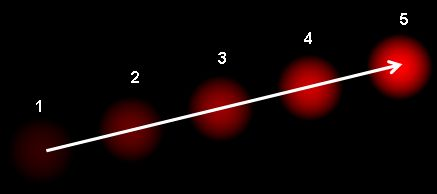
\includegraphics[width=80mm]{Pictures/opticflow.jpg}
\caption{Arrow showing optical flow}
\end{figure}



Optical flow works on several assumptions:
\begin{enumerate}
    \item The pixel intensities of an object do not change between consecutive frames.
    \item The motion between consecutive frames is small. 
    \item Neighbouring pixels have similar motion.
\end{enumerate}

Consider a pixel $I(x,y,t)$  in first frame.It moves by distance ($dx,dy$) in next frame taken after $dt$ time. So since those pixels are the same and intensity does not change, we can say, 

\[I(x,y,t)=I(x+dx,y+dy,t+dt)\]
Then taking taylor series approximation of right-hand side and neglecting higher order terms 


\[I(x,y,t) =I(x,y,t)+\frac{\partial I}{\partial x}dx+\frac{\partial I}{\partial y}dy+\frac{\partial I}{\partial t}dt \] 

\[\frac{\partial I}{\partial x}dx+\frac{\partial I}{\partial y}dy+\frac{\partial I}{\partial t}dt = 0 \]

Dividing by \(dt\) we get 
\begin{equation} \label{eq1}
f_{x}u+f_{y}v+f_{t}=0
\end{equation}

where 
    \[f_{x}=\frac{\partial f}{\partial x} \quad f_{y}=\frac{\partial f}{\partial y} \quad u=\frac{dx}{dt}\quad v=\frac{dy}{dt}\]

Above equation is called Optical Flow equation. In it, we can find \(f_{x}\) and \(f_{y}\), they are image gradients. Similarly \(f_{t}\) is the gradient along time. But ($u,v$) is unknown. We cannot solve this one equation with two unknown variables. So several methods are provided to solve this problem and one of them is Lucas-Kanade.


\subsection{Lucas-Kanade method}
We have seen an assumption before, that all the neighbouring pixels will have similar motion. Lucas-Kanade method takes a 3x3 patch around the point. So all the 9 points have the same motion. We can find $(f_{x},f_{y},f_{t})$ for these 9 points. So now our problem becomes solving 9 equations with two unknown variables which is over-determined.Those 9 equations are represented in a matrix and using the concept of psuedo inverse as shown below.

\begin{align*}
    AU = F\\
    A^{T}AU = A^{T}F\\
    U = (A^{T}A)^{-1}A^{T}F\\
\end{align*}
where
\[
A = \begin{bmatrix}
f_{x1} & f_{y1} \\
f_{x2} & f_{y2} \\
\vdots & \vdots \\
f_{x9} & f_{y9} 

\end{bmatrix} \quad
U = \begin{bmatrix}
u\\
v
\end{bmatrix} \quad
F = \begin{bmatrix}
-f_{t1}\\
-f_{t2}\\
\vdots\\
-f_{t9}
\end{bmatrix}
\]
Below is the final solution which is two equation-two unknown problem and solve to get the solution.
\[
\begin{bmatrix}
u \\ v \end{bmatrix} = \begin{bmatrix} \sum_{i}{f_{x_i}}^2 & \sum_{i}{f_{x_i} f_{y_i} } \\ \sum_{i}{f_{x_i} f_{y_i}} & \sum_{i}{f_{y_i}}^2 \end{bmatrix}^{-1} \begin{bmatrix} - \sum_{i}{f_{x_i} f_{t_i}} \\ - \sum_{i}{f_{y_i} f_{t_i}} \end{bmatrix}\]


The good thing was this was all already implemented in \textbf{open cv}.Finally note that this derivation is valid only for detecting small motions.For our purpose,the motion between two consecutive frames is very less.Hence this method can be safely applied.If we obtain ($u,v$) for every pixel in the image,then it is called dense optical flow and we have used dense optical flow in the proposed approach.

There are several other algorithms proposed to solve optical flow.you can refer them here\cite{Optical}


\section{Histogram of Optical flow}
A feature descriptor is a representation of an image or an image patch that simplifies the image by extracting useful information and throwing away extraneous information.Typically, a feature descriptor converts an image of size width x height x 3 (channels) to a feature vector / array of length n.Histogram of Optical Flow (HOF) is one such descriptor.In the case of the HOG feature descriptor, the input image is of size $h * w * 3$ and the output feature vector is of length $ h * w * 9 / 64 $.

In the HOF feature descriptor, the distribution ( histograms ) of directions of optical flow are used as features.Since, we are trying to cluster motions,optical flow serves as good feature for capturing motion.The following shows the steps in the calculation of HOF descriptor.

\textbf{Step 1 : Calculate Optical Flow}

To calculate a HOF descriptor, we need to first calculate the optical flow; after all, we want to calculate the histogram of optical flow.To calculate the optical flow, use the methods described above.Now we get two components ($u,v$) foe every pixel by using the optical flow.

\textbf{Step 2 : Calculate Histogram of Gradients in \begin{math}8*8\end{math} cells}

In this step, the image is divided into \begin{math}8*8\end{math} cells and a histogram of optical flow is calculated for each \begin{math}8*8\end{math} cells.One of the important reasons to use a feature descriptor to describe a patch of an image is that it provides a compact representation.

An \begin{math}8*8\end{math} image patch contains \begin{math}8*8*3\end{math} = 192 pixel values. The optical flow of this patch contains 2 values ( magnitude and direction ) per pixel which adds up to \begin{math}8*8*2\end{math} = 128 numbers. By the end of this section we will see how these 128 numbers are represented using a 9-bin histogram which can be stored as an array of 9 numbers. Not only is the representation more compact,calculating a histogram over a patch makes this representation more robust to noise. Individual optical flow may have noise, but a histogram over \begin{math}8*8\end{math} patch makes the representation much less sensitive to noise.

The histogram is essentially a vector ( or an array ) of 18 bins ( numbers ).First convert the optical flow ($u,v$) of every pixel into polar coordinates.The bins can be made using following two techniques

\textbf{Interval Binning}


In this technique, the bins are considered as intervals 0 - 20 , 20 - 40 ... , 340 - 360. For every pixel in the \begin{math}8*8\end{math} patch a bin is selected based on the direction, and the vote ( the value that goes into the bin ) is selected based on the magnitude.

\newpage

\textbf{Weighted Binning}

In this technique, The histogram contains 18 bins corresponding to angles 0, 20, 40 … 160. For every pixel in the \begin{math}8*8\end{math}. Depending on the direction, the magnitude is split across at most two bins depending on the distance of direction from bin angle.An illustration of this is shown below.

\begin{figure} [!htbp]
\centering
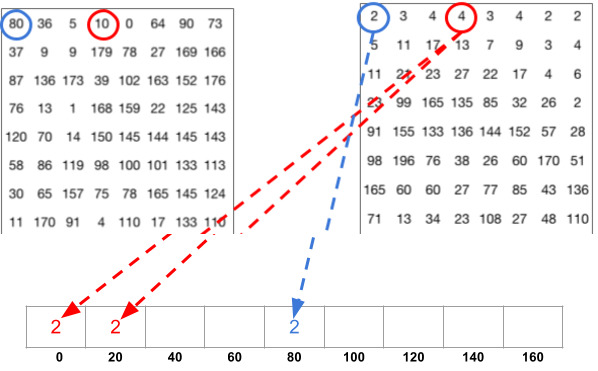
\includegraphics[width=80mm]{Pictures/HOF.jpg}
\caption{Weighted Binning illustration}
\end{figure}

Let’s first focus on the pixel encircled in blue. It has an angle ( direction ) of 80 degrees and magnitude of 2. So it adds 2 to the 5th bin. The optical flow at the pixel encircled using red has an angle of 10 degrees and magnitude of 4. Since 10 degrees is half way between 0 and 20, the vote by the pixel splits evenly into the two bins.

\textbf{Step 4 : \begin{math}16*16\end{math} Block Normalization}

In order the descriptor to be independent of lighting variations, we would like to “normalize” the histogram so they are not affected by lighting variations.A \begin{math}16*16\end{math} block has 4 histograms which can be concatenated to form a \begin{math}36 * 1\end{math} element vector and it will be normalized.The window is then moved by 8 pixels and a normalized \begin{math}36 * 1\end{math} vector is calculated over this window and the process is repeated.After doing this,all the bins are concatenated to form the final feature vector. 

But for our motion clustering, this step didn't worked well(Accuracy without this step was good).Hence we just didn't up to step 3.Let us say for each frame the HOF vector is of size x. If a motion has f frames the feature vector size will be of size $f*x$. Since it depends on number of frames,feature vector for each motion may not be of same size.










\section{Dynamic Time Warping (DTW) }

The distance between two point \({x}=[x_{1}, x_{2}, ..., x_{n}]\) and \({y}=[y_{1}, y_{2}, ..., y_{n}]\) in a n-dimensional space can be computed via the Euclidean distance: 
\[dist(\mathbf{x},\mathbf{y})=\|\mathbf{x}-\mathbf{y}\|=\sqrt{(x_1-y_1)^2+(x_2-y_2)^2+\cdots+(x_n-y_n)^2}.\]

However, if the length of \(\mathbf{x}\) is different from \(\mathbf{y}\), then we cannot use the above formula to compute the distance. Instead, we need a more flexible method that can find the best mapping from elements in \(\mathbf{x}\) to those in \(\mathbf{y}\) in order to compute the distance.

The goal of \textbf{dynamic time warping} (DTW for short) is to find the best mapping with the minimum distance by the use of DP. The method is called \textbf{"time warping"} since both x and y are usually vectors of time series and we need to compress or expand in time in order to find the best mapping.

Let t and r be two vectors of lengths m and n, respectively. The goal of DTW is to find a mapping path \( \{(p_1, q_1), (p_2, q_2), ..., (p_k, q_k)\} \)  such that the distance on this mapping path \textbf{\( \sum_{i=1}^k |t(p_i)-r(q_i)|\)} is minimized, with the following constraint:
\begin{itemize}
    \item The ordering should be preserved meaning if i is mapped with j then i-1 can be mapped with any index until j but not beyond j.This local constraint guarantees that the mapping path is monotonically non-decreasing in its first and second arguments. Moreover, for any given element in t, we should be able to find at least one corresponding element in r, and vice versa.  
\end{itemize}

\begin{figure} [!htbp]
\centering
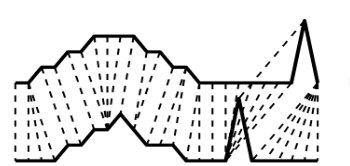
\includegraphics[width=80mm]{Pictures/dtw.png}
\caption{Figure showing the mapping obtained by DTW}
\end{figure}


\subsection{Solving DTW}

we can solve it using the following dynamic programming(DP) approach.

\begin{enumerate}
    \item \textbf{Optimum-value function} : Define $D(i,j)$ as the DTW distance between $t(1:i)$ and $r(1:j)$, with the mapping path starting from $(1,1)$ to $(i,j)$
    
    \item \textbf{Recursion} :
    \[D(i, j)=|t(i) - r(j)| + min \left\{\begin{matrix} D(i-1, j)\\D(i-1, j-1)\\D(i, j-1) \end{matrix}\right\},\]
    
     with the initial condition \(D(1, 1)=|t(1)-r(1)|\)
    \item \textbf{Final answer} : $D(m,n)$
\end{enumerate}

If we want to know the optimum mapping path in addition to the minimum distance, we may want to keep the optimum fan-in of each node. Then at the end of DP, we can quickly back track to find the optimum mapping path between the two input vectors. 

There are many attempts made to make DTW run faster.you can refer \cite{DTW} to know about a faster version of DTW.

\subsection{Applications}
Dynamic time warping is mainly used in speech recognition,since speech is very sensitive for variations in time,but the technique has proved to be useful for many other applications like gesture recognition, robotics, data mining,hand writing recognition etc


For our purpose,we used DTW for measuring similarity between motions.As we stated earlier that each motion is represented by a feature vector of different sizes.Hence we use DTW to compare these unequal sized feature vectors.Everything remains same except the t,r vectors which in our case are not simple vectors but vector of vectors.This will be explained in detail in the coming chapters.

\section{Spectral Clustering}
The goal of spectral clustering is to cluster data that is connected but not necessarily compact or clustered within convex boundaries.It very often outperforms traditional clustering algorithms such as the k-means algorithm.

\begin{figure} [!htbp]
\centering
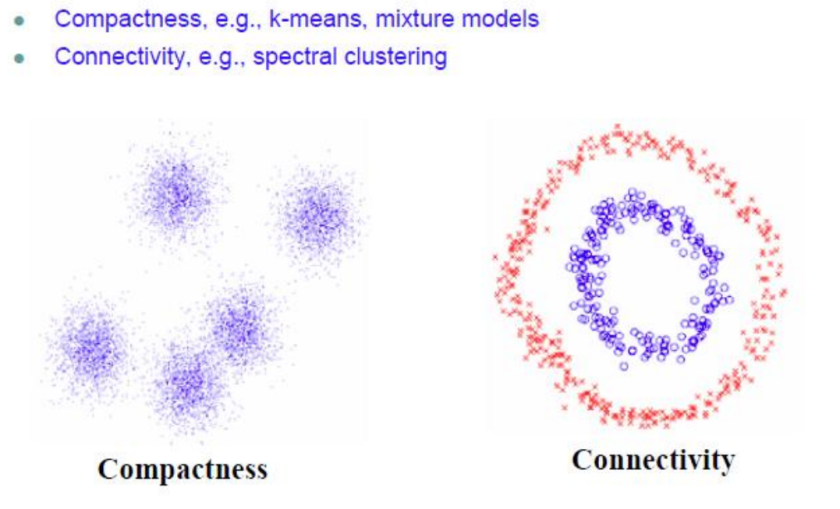
\includegraphics[width=80mm]{Pictures/spec.png}
\caption{Example explaining two properties of data}
\end{figure}

\subsection{Basic Idea}
\begin{itemize}
    \item Spectral clustering models the objective function as a graph spectrum problem and solves it with the known linear algebra techniques.
    \item It connects the objective function to one of the following  property of graph laplacian and solves it in place of minimizing objective function.
\end{itemize}

For every vector $f \in R^{n}$ we have

\[f^{'}Lf = \frac{1}{2}\sum_{i,j=1}^{n}w_{ij}\left (f_{i} - f_{j} \right )^{2}\]
where 
\[ L = D - W  , \quad \text{W is the adjacency Matrix} \]
\[d_{i} = \sum_{j=1}^{n}w_{ij} \]
\centerline{D is a diagonal Matrix with $d_{i}$  as diagonal}

\subsection{Algorithm}
\begin{enumerate}
    \item \textbf{Input} : Similarity matrix $W \in R^{n*n}$ , number k of clusters to construct
    \item Compute the unnormalized Laplacian $L$.
    \item Compute the first k eigenvectors ($u_{1},u_{2},\dots,u_{k}$) of $L$.
    \item Let $U \in R^{n*k}$ be the matrix containing the vectors $u_{1},u_{2},\dots,u_{k}$ as columns.
    \item Let $i = 1\dots n$ let $y_{i} \in R^{k}$ be be the vector corresponding to the $i_{th}$ row of U
    \item Cluster the points $(y_{i})_{i=1,\dots,n}$ in $R^{k}$ with k-means clustering algorithm into $C_{1},\dots,C_{k}$ clusters.
    \item \textbf{Output} : Clusters $A_{1},A_{2},\dots,A_{k}$ with $A_{i} = \{j | y_{i} \in C_{j} \}$
    
    
\end{enumerate}


\subsection{Objective Function}
The following is the Objective function the spectral clustering is trying to minimize
\begin{figure} [!htbp]
\centering
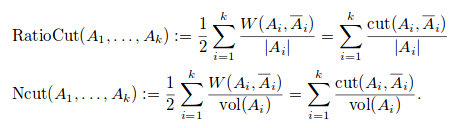
\includegraphics[width=100mm]{Pictures/obj.png}
\caption{Objective Function}
\end{figure}

Intuitively this function is trying to minimize the  sum of crossing edges between clusters while trying to maximize the within cluster edges.Note that here edge weight represent similarity.In other words,it is trying to maximize within cluster similarity while minimizing across cluster similarity.

\subsection{How the algorithm is minimizing the above Function }
This section shows how graph laplacian is related to the above objective function and hence we can minimize the laplacian property instead of that objective function.

\subsubsection{Approximating Ratio Cut for K = 2}
\begin{figure} [!htbp]
\centering
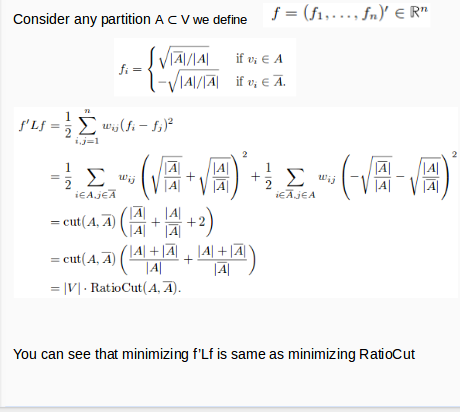
\includegraphics[width=100mm]{Pictures/k=2.png}
\caption{Figure showing how Laplacian property related to RatioCut}
\end{figure}

Finally we should minimize the below equation to minimize the objective function
\begin{figure} [!htbp]
\centering
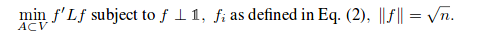
\includegraphics[width=120mm]{Pictures/minim.png}
\end{figure}

This is a discrete optimization problem but it is NP Hard.Relaxing f to take real values makes it solvable.By the Rayleigh-Ritz theorem, 
the solution to this is eigenvector corresponding to the second smallest eigenvalue of L.
\subsubsection{Approximating Ratio Cut for K \texorpdfstring{$>$}{Lg} 2}
\begin{figure}[H]
\centering
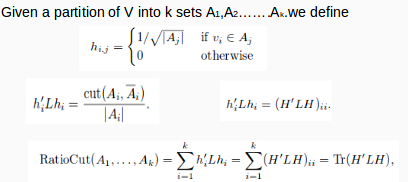
\includegraphics[width=100mm]{Pictures/k>2_half.png}
\end{figure}

The final minimization problem is
\begin{figure} [!htbp]
\centering
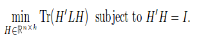
\includegraphics[width=60mm]{Pictures/spec2.png}
\end{figure}

By the Rayleigh-Ritz theorem,the solution is given by choosing H as the matrix which contains the first k eigen vectors of L as columns.So,for this reason we are calculating first k eighen vectors in the algorithm.we can refer \cite{Spectral1} for more indepth details on spectral clustering.


\section{Support Vector Machine}

A Support Vector Machine (SVM) is a supervised machine learning algorithm that can be employed for both classification and regression purposes. SVMs are more commonly used in classification problems.SVMs are based on the idea of finding a hyperplane that best divides a dataset into two classes, as shown in the image below.

\begin{figure} [!htbp]
\centering
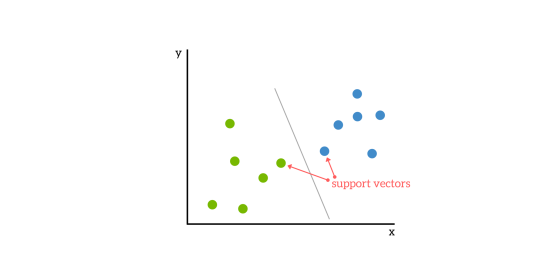
\includegraphics[width=100mm]{Pictures/svm1.png}
\caption{Figure demonstrating hyperplane}
\end{figure}

\subsection{Support Vectors}

Support vectors are the data points nearest to the hyperplane, the points of a data set that, if removed, would alter the position of the dividing hyperplane. Because of this, they can be considered the critical elements of a data set.

\subsection{HyperPlane}

As a simple example, for a classification task with only two features (like the image above), you can think of a hyperplane as a line that linearly separates and classifies a set of data.

Intuitively, the further from the hyperplane our data points lie, the more confident we are that they have been correctly classified. We therefore want our data points to be as far away from the hyperplane as possible, while still being on the correct side of it.So when new testing data is added, whatever side of the hyperplane it lands will decide the class that we assign to it.


\subsection{Finding the right hyperplane}

The distance between the hyperplane and the nearest data point from either set is known as the \textbf{margin}. The goal is to choose a hyperplane with the greatest possible margin between the hyperplane and any point within the training set, giving a greater chance of new data being classified correctly.

\begin{figure} [!htbp]
\centering
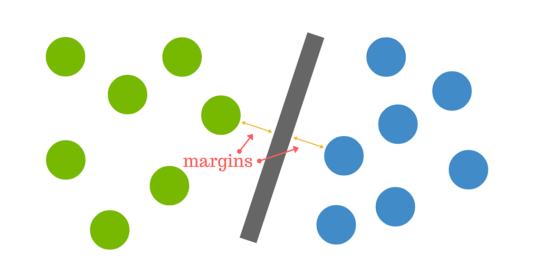
\includegraphics[width=100mm]{Pictures/svm2.png}
\caption{Figure demonstrating margin}
\end{figure}

\subsection{Linearly non separable data}

We will transform the axes and convert the data into linearly separable.The transformation of data is done using concept called \textbf{kernels}.The below figures demonstrates how the transformation is done.

\begin{figure} [!htbp]
\centering
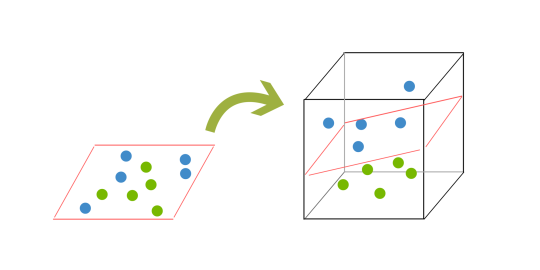
\includegraphics[width=100mm]{Pictures/svm3.png}
\caption{Figure demonstrating kernels}
\end{figure}

For mathematical foundations of SVM, refer \href{http://cs229.stanford.edu/notes/cs229-notes3.pdf}{CS229 Lecture notes}. 

\section{K- Nearest Neighbour (KNN)}

k-nearest neighbors algorithm (k-NN) is a non-parametric method used for classification and regression.In this supervised learning technique,there is no training phase.when a new data point come,it will be assigned the class of training data point which is closest to the new data point.The "closest" is defined as per application requirements.In our context the closest is defined using the measure DTW.




\section{Accuracy Measure (Rand Index)}
In order to evaluate the results obtained by our algorithm,we have used \textbf{rand index} as a evaluation measure for computing accuracy.

If C is a ground truth class assignment and K the clustering,then let:
\begin{itemize}
    \item a, the number of pairs of elements that are in the same set in C and K
    \item b, the number of pairs of elements that are in different sets in both  C and K
\end{itemize}
\[ RI = \frac{a + b}{\binom{n_{samples}}{2}}\]
















